\documentclass[t]{beamer}
% Theme
\usetheme[sectionpage=progressbar]{metropolis}

% Informationen
\title{Kolloquiumsvortrag zur Bachelorarbeit - Erklärbarkeit und Visualisierung von Graph Codes mittels generativer KI}
\subtitle{Bachelorarbeit an der Fernuniversität in Hagen}
\author{Jens Andress}
\date{\today}
\institute{Lehrgebiet Multimedia und Internetanwendungen}

\begin{document}

\maketitle

\begin{frame}{Inhaltsverzeichnis}
  \tableofcontents

  \pagenumbering{gobble}
\end{frame}

\section{Einleitung}

\metroset{block=fill}

\begin{frame}{Einleitung}

  \begin{exampleblock}{Allgemeine kompakte Themenbeschreibung}
    In dieser Arbeit wurde untersucht, inwieweit generative KI geeignet ist, präzise und für Menschen verständliche / intuitive Erklärungen aus Graph Codes zu generieren.
  \end{exampleblock}

\end{frame}

\begin{frame}{Einleitung}

  \begin{block}{Mehrwert (für Benutzer)}
    \begin{itemize}
      \item Präzise / individuellere Erklärungen durch generative KI.
      \item Andere Formen von Erklärungen (Bild, aber auch andere Formen denkbar).
      \item Überblick über / Ordnung von Zusammenhängen zwischen Merkmalen.
      \item Barrierefreiheit durch generative KI (Screen Readers).
      \item Zeitersparnis.
    \end{itemize}
  \end{block}

\end{frame}

\begin{frame}{Einleitung}
  \begin{block}{Problembereich (Erklärbarkeit)}
    \begin{itemize}
      \item<+-> Verfahren zur Erklärbarkeit von Prozessen des MMIR basieren auf statischen und rein mathematischen Ansätzen.
      \item<+-> Einzige Form von Erklärungen, die das GMAF bietet, sind (eingeschränkte) textuelle Erklärungen.
      \item<+-> GMAF bietet keine Möglichkeit für Benutzer unterschiedliche Anwendungsfälle in Bezug auf Erklärungen abdecken zu können.
      \item<+-> GMAF bietet nur grobe Möglichkeiten zur Anpassungen der generierten Erklärungen.
    \end{itemize}
  \end{block}
\end{frame}

\begin{frame}{Einleitung}
  \begin{alertblock}{Problemstellung PB 1.}
    Generative KI ist aktuell nicht für die Erklärbarkeit von Prozessen des MMIR nutzbar.
  \end{alertblock}
\end{frame}

\begin{frame}{Einleitung}
  \begin{block}{Problembereich (Integration)}
    \begin{itemize}
      \item<+-> GMAF besitzt keine Anbindung von Systemen generativer KI.
      \item<+-> GMAF besitzt keine Möglichkeit die in MMIR-Prozessen identifizierten Merkmale in gültige und geeignete Eingabedaten für Systeme generativer KI zu überführen.
    \end{itemize}
  \end{block}
\end{frame}

\begin{frame}{Einleitung}
  \begin{alertblock}{Problemstellung PB 2.}
    Das GMAF bietet keine Integration generativer KI.
  \end{alertblock}
\end{frame}

\begin{frame}{Einleitung}

  \begin{exampleblock}{Allgemeine Zielsetzung}
    Die im GMAF implementierten Konzepte zur Erklärung von Prozessen des MMIR sollen durch \textbf{generative KI} abgelöst werden, um \textbf{bessere Erklärungen}, sowie \textbf{andere Formen von Erklärungen} zu ermöglichen.
  \end{exampleblock}

\end{frame}

\begin{frame}{Einleitung}
  \textbf{Problemstellungen}

  \begin{alertblock}{Problemstellung PB 1.}
    Generative KI ist aktuell nicht für die Erklärbarkeit von Prozessen des MMIR nutzbar.
  \end{alertblock}

  \begin{alertblock}{Problemstellung PB 2.}
    Das GMAF bietet keine Integration generativer KI.
  \end{alertblock}
  Daraus wurden folgende Forschungsfragen formuliert...
\end{frame}

\begin{frame}{Einleitung}
  \textbf{Forschungsfragen}

  \begin{alertblock}{Forschungsfrage FF 1.}
    Kann generative KI für die Erklärbarkeit von Prozessen des MMIR genutzt werden?
    \\
    \onslide<2>{
      $\rightarrow$ FZ 1: Erklärbarkeit von MMIR mittels generativer KI.
    }
  \end{alertblock}

  \begin{alertblock}{Forschungsfrage FF 2.}
    Wie lässt sich generative KI in das GMAF integrieren?
    \\
    \onslide<2>{
      $\rightarrow$ FZ 2: Integration generativer KI in das GMAF.
    }
  \end{alertblock}
  In jedem Kapitel werden diese Forschungsfragen durch entsprechende Forschungsziele abgearbeitet.
  Diese Forschungsziele sind also als Ankerpunkte dieser Arbeit zu verstehen.
\end{frame}

\section{Stand der Wissenschaft und Technik}

% Forschungsziel 1.1/O

\begin{frame}{Forschungsziel FZ 1.1/O}
  \begin{block}{Was wurde erarbeitet / recherchiert?}
    \begin{itemize}
      \item<+-> Grundlegende Technologien: GMAF, MMFG, Graph Codes.
      \item<+-> Grundlegende Begrifflichkeiten zu generativer KI.
      \item<+-> Aktuelle Systeme / Überblick zu generativer KI.
      \item<+-> Diskussion von Systemen generativer KI.
    \end{itemize}
  \end{block}
\end{frame}

\begin{frame}{Forschungsziel FZ 1.1/O}
  \begin{block}{Gewonnene Erkenntnisse}
    \begin{itemize}
      \item<+-> Erste offene Herausforderung \textbf{OH 1.1}.
      \item<+-> Auswahl von vorgestellten Systemen generativer KI \\
      ({\color{red} GPT-x {\color{black} u.} Dall-E 2 {\color{black} von} OpenAI}).
      \item<+-> Zweite offene Herausforderung \textbf{OH 1.2}.
    \end{itemize}
  \end{block}
  \only<1>{
    \begin{block}{OH 1.1 - Erklärbarkeit durch generative KI}
      Einsatz von generativer KI als Ersatz bzw. Alternative zur statistischen und rein mathematischen Vorgehensweise, um Erklärungen zu generieren.
    \end{block}
  }
  \only<3>{
    \begin{block}{OH 1.2 - Benutzerschnittstelle}
      %Sollen diese Systeme im Rahmen des GMAF sinnvoll eingesetzt werden, um Erklärungen generieren zu können, so müssen Anwendern des GMAF durch eine Benutzerschnittstelle geeignete Interaktionsmöglichkeiten mit diesen Systemen geboten werden.
      Sinnvoller Einsatz von Systemen generativer KI setzt eine Benutzerschnittstelle mit geeigneten Interaktionsmöglichkeiten voraus.
    \end{block}
  }
\end{frame}

% Forschungsziel 2.1/O

\begin{frame}{Forschungsziel FZ 2.1/O}
  \begin{block}{Was wurde erarbeitet / recherchiert?}
    \begin{itemize}
      \item<+-> Integrationsmöglichkeiten von Graph Codes.
      \item<+-> Integrationsmöglichkeiten von ausgewählten Systemen generativer KI.
    \end{itemize}
  \end{block}
\end{frame}

\begin{frame}{Forschungsziel FZ 2.1/O}
  \begin{block}{Gewonnene Erkenntnisse}
    \begin{itemize}
      \item<+-> Übersicht über Komponenten im GMAF.
      \item<+-> Erste offene Herausforderung \textbf{OH 2.1}.
      \item<+-> Übersicht über Endpunkte der Schnittstelle von OpenAI.
      \item<+-> Zweite offene Herausforderung \textbf{OH 2.2}.
    \end{itemize}
  \end{block}
  \only<2>{
    \begin{block}{OH 2.1 - Transformieren von Graph Codes}
      Umwandlung von Graph Codes in eine passende Eingabeform für Systeme generativer KI.
    \end{block}
  }
  \only<4>{
    \begin{block}{OH 2.2 - Integration generativer KI}
      Zum Zeitpunkt des Verfassens dieser Arbeit existiert keine Integration der von OpenAI angebotenen Systeme generativer KI im GMAF.
    \end{block}
  }
\end{frame}

\section{Modellierung}

% Forschungsziel 1.1/O

\begin{frame}{Forschungsziel FZ 1.2/TB}
  \begin{block}{Was wurde erarbeitet / modelliert?}
    \begin{itemize}
      \item<+-> Erklärbarkeit durch generative KI.
      \item<+-> Anwendungsfälle.
      \item<+-> Wireframe für Benutzerschnittstelle.
      \item<+-> Mechanismen.
      \item<+-> UML-Sequenzdiagramme.
    \end{itemize}
  \end{block}
\end{frame}

\begin{frame}{Forschungsziel FZ 1.2/TB}
  \begin{block}{Gewonnene Erkenntnisse}
    \begin{itemize}
      \item<+-> Behandlung erster offener Herausforderung.
      \item<+-> Grundsätzliches Modell für Benutzerschnittstelle.
      \item<+-> Behandlung zweiter offener Herausforderung.
      \item<+-> An Anwendungsfall beteiligte Komponenten.
      \item<+-> Abläufe und Interaktion zwischen Komponenten.
    \end{itemize}
  \end{block}
\end{frame}

% Forschungsziel 2.1/O

\begin{frame}{Forschungsziel FZ 2.2/TB}
  \begin{block}{Was wurde erarbeitet?}
    \begin{itemize}
      \item<+-> Transformation von Graph Codes.
      \item<+-> Einbindung von Systemen generativer KI.
    \end{itemize}
  \end{block}
\end{frame}

\begin{frame}{Forschungsziel FZ 2.2/TB}
  \begin{block}{Gewonnene Erkenntnisse}
    \begin{itemize}
      \item<+-> Konzepte zur Transformation von Graph Codes.
      \item<+-> Behandlung erster offener Herausforderung.
      \item<+-> Konzepte zur Integration von Systemen generativer KI.
      \item<+-> Behandlung zweiter offener Herausforderung.
    \end{itemize}
  \end{block}
\end{frame}

\section{Implementierung}

\begin{frame}{Implementierung}
  Die folgenden Abbildungen zeigen Screenshots der entwickelten prototypischen Proof-of-Concept Implementierung.
\end{frame}

\begin{frame}{Implementierung - Screenshots}

  \begin{figure}
    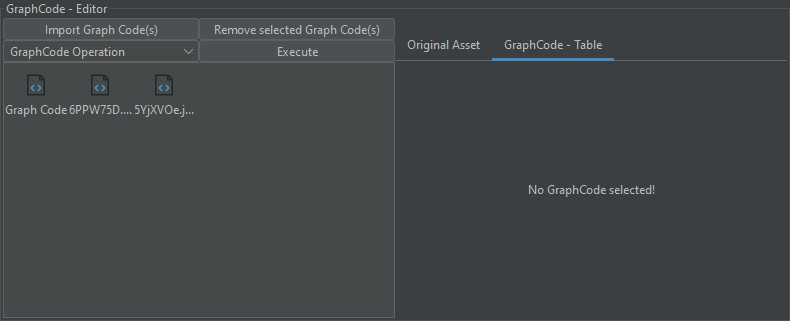
\includegraphics[width=\textwidth]{images/left_no_sel}
    \caption{Kein Graph Code ausgewählt.}
  \end{figure}

\end{frame}

\begin{frame}{Implementierung - Screenshots}

  \begin{figure}
    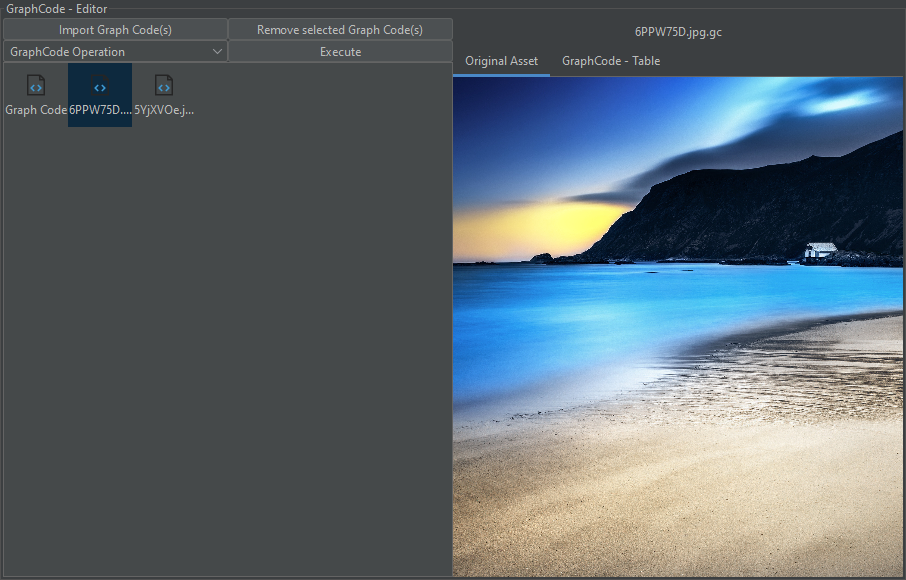
\includegraphics[width=0.9\textwidth]{images/left_sel_original}
    \caption{Graph Code ausgewählt, Darstellung der originalen Datei.}
  \end{figure}

\end{frame}

\begin{frame}{Implementierung - Screenshots}

  \begin{figure}
    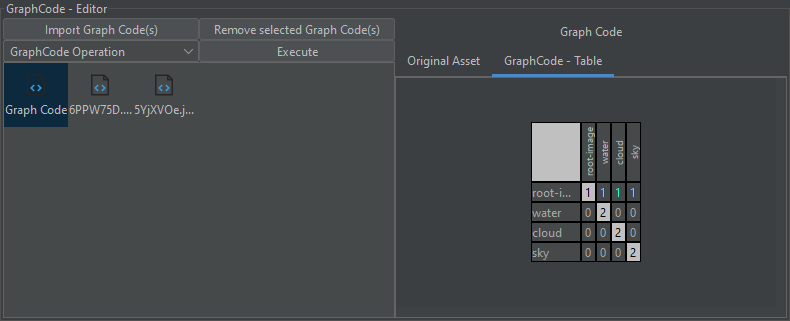
\includegraphics[width=\textwidth]{images/left_sel}
    \caption{Graph Code ausgewählt, tabellarische Darstellung des Graph Codes.}
  \end{figure}

\end{frame}

\begin{frame}{Implementierung - Screenshots}

  \begin{figure}
    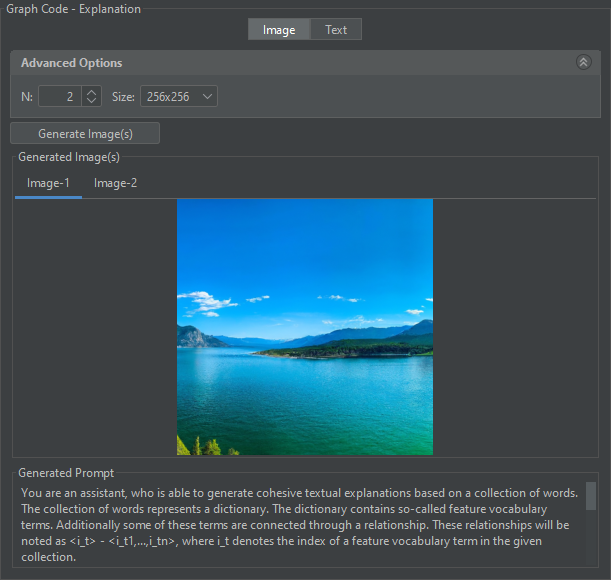
\includegraphics[width=0.6\textwidth]{images/right_img_two_exps_1}
    \caption{Erstes Bild zu ausgewähltem Graph Code generiert.}
  \end{figure}

\end{frame}

\begin{frame}{Implementierung - Screenshots}

  \begin{figure}
    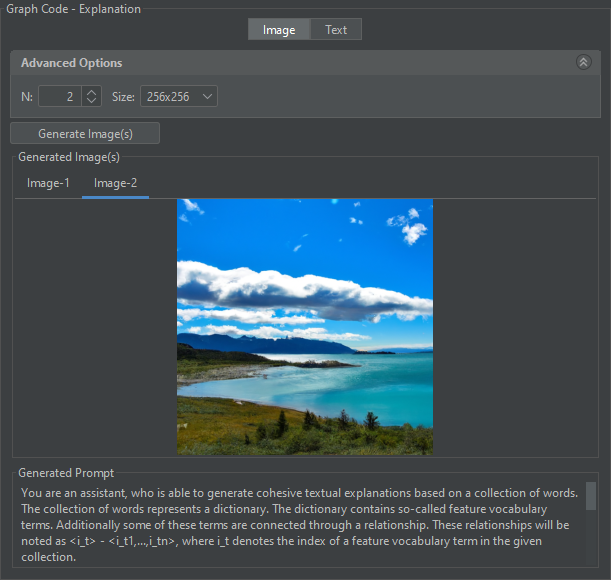
\includegraphics[width=0.6\textwidth]{images/right_img_two_exps_2}
    \caption{Zweites Bild zu ausgewähltem Graph Code generiert.}
  \end{figure}

\end{frame}

\begin{frame}{Implementierung - Screenshots}

  \begin{figure}
    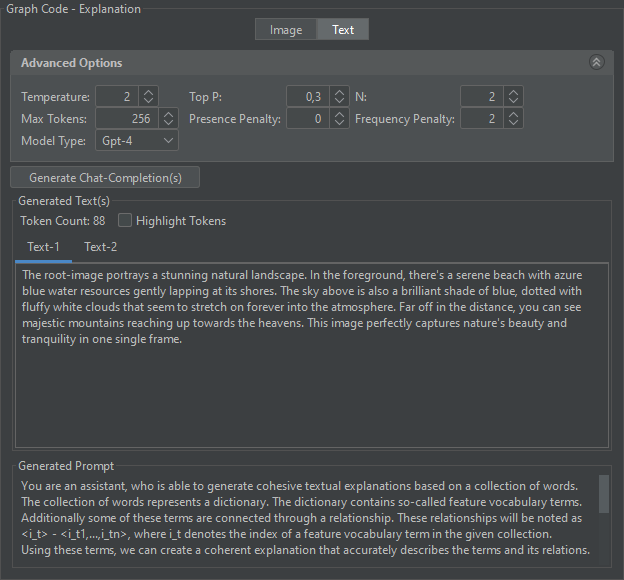
\includegraphics[width=0.6\textwidth]{images/right_text_two_exps_1}
    \caption{Erster Text zu ausgewähltem Graph Code generiert.}
  \end{figure}

\end{frame}

\begin{frame}{Implementierung - Screenshots}

  \begin{figure}
    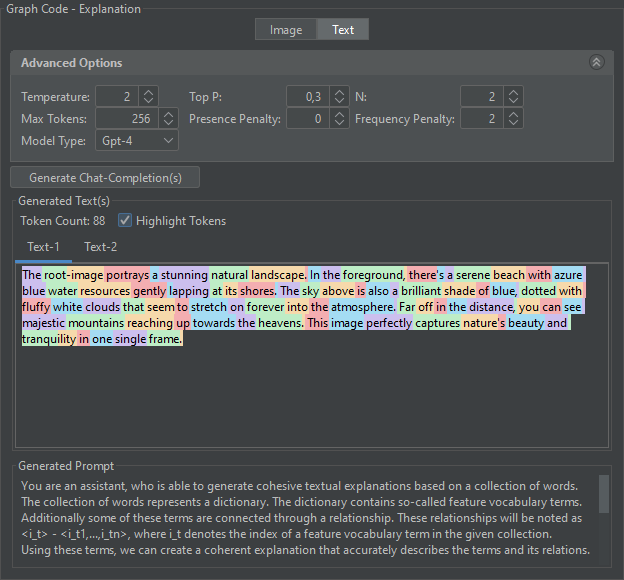
\includegraphics[width=0.6\textwidth]{images/right_text_two_exps_1_high}
    \caption{Hervorheben von Tokens beim ersten generierten Text.}
  \end{figure}

\end{frame}

\begin{frame}{Implementierung - Screenshots}

  \begin{figure}
    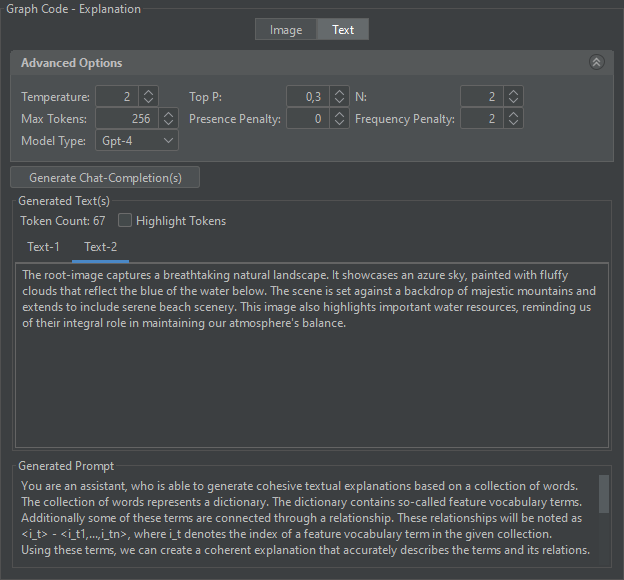
\includegraphics[width=0.6\textwidth]{images/right_text_two_exps_2}
    \caption{Zweiter Text zu ausgewähltem Graph Code generiert.}
  \end{figure}

\end{frame}

\section{Zusammenfassung}

\begin{frame}{Zusammenfassung}

  \begin{block}{Herausforderungen}
    Generativer KI Aufgaben mittels Instruktionen zu vermitteln (Zufälligkeitsfaktor, jede generierte Antwort kann im Wortlaut individuell sein).
  \end{block}

  \begin{block}{Stolpersteine}
    Keine Stolpersteine während der Bearbeitung der Arbeit erfahren.
  \end{block}

\end{frame}

\end{document}
